
% =========================================================
% Scientific Reports — submission-ready (sn-jnl)
% NO‑CAL reproducibility note for hydrogen ground state
% Author: LEE YOUNG JAE (Independent Researcher)
% Email: rego093@naver.com
% =========================================================
\documentclass[sn-std,Numbered]{sn-jnl} % Springer Nature master class
\jyear{2025}

\title{A no‑calibration reproducibility kit for the hydrogen ground state:
sealed scales, 1\% external checks, and cross‑platform validation}

\author*[1]{\fnm{YOUNG JAE} \sur{LEE}}\email{rego093@naver.com}
\affil*[1]{\orgdiv{Independent Researcher}, \orgaddress{\city{Daegu}, \country{Republic of Korea}}}

\abstract{
We present a \textbf{no‑calibration (NO‑CAL)} reproducibility kit for the hydrogen ground state that (i) derives Hartree and Bohr scales directly from SI‑defined constants, (ii) \textbf{seals} them in a JSON file with a pinned SHA256 hash cited in‑text, and (iii) verifies two \textbf{1\% external criteria} via a separate \texttt{verify.py} returning \texttt{exit(0|1)} and supporting \textbf{negative‑control re‑execution}. A cross‑platform log aggregates OS/Python/NumPy versions, the sealed hash, and results. On a Linux reference run we obtain $E_{1,\mathrm{eV}}=13.6056931$ and $a_{\mathrm{H}}=0.5291772109$~\AA, achieving $R7=5.05\times10^{-5}$ and $R8=3.99\times10^{-5}$. The manuscript anchors integrity with the seal hash \texttt{cf3c1684f369a1f5aa6b7e40384002fa9e807d98e27807c4d556c14cb06f4453} and provides all artifacts and scripts. This \emph{soundness‑first, artifacts‑complete} package aligns with Scientific Reports’ validity‑based editorial policy and data‑availability requirements.
}

\keywords{reproducibility, no calibration, sealed scales, data availability, verification, exit code}

\maketitle
\graphicspath{{figs/}{tables/}}

\section{Introduction}
Reproducibility benefits from three pillars: \textbf{sealed scales} (no hidden fitting), \textbf{externally checkable targets with explicit tolerances}, and \textbf{deterministic scripts} returning programmatic pass/fail.
Hydrogen is chosen because key quantities follow from the non‑relativistic Coulomb model using SI‑defined constants. Our kit operationalizes these principles with minimal assumptions and no calibration (“NO‑CAL”), focusing on \emph{technical soundness and transparency} rather than impact claims \cite{Griffiths2018,Sakurai2017,SIbrochure2019}.

\section{Results}
\subsection{Main external 1\% checks}
With the sealed scales, we compute $E_{1,\mathrm{eV}}$ and $a_{\mathrm{H}}$ and verify:
\[
R7=\frac{|E_{1,\mathrm{eV}}-13.6057|}{0.01\times 13.6057}\le 1,\quad
R8=\frac{|a_{\mathrm{H}}-0.529177|}{0.01\times 0.529177}\le 1.
\]
Table~\ref{tab:main} summarizes the main run (Linux reference).

\begin{table}[t]
\caption{Main external checks (1\% criteria).}\label{tab:main}
\centering
\begin{tabular}{lccccc}
\toprule
Run & $E_{1,\mathrm{eV}}$ & $a_{\mathrm{H}}$ (\AA) & R7 & R8 & PASS \\
\midrule
Linux(ref) & 13.6056931 & 0.5291772109 & 5.05e-05 & 3.99e-05 & Yes \\
macOS & (to be appended) & (to be appended) & -- & -- & -- \\
Windows & (to be appended) & (to be appended) & -- & -- & -- \\
\bottomrule
\end{tabular}
\end{table}


\subsection{Negative controls (re‑execution)}
We re‑execute the same analytical pipeline with \texttt{--gate-off} \{\texttt{EM\_c}, \texttt{JIN}, \texttt{Gamma3}\}. Each gate‑off run fails by construction, confirming that success depends on physically meaningful gates rather than post‑hoc overrides. See Table~\ref{tab:neg}.

\begin{table}[t]
\caption{Negative controls (same pipeline, gate-off re-execution).}\label{tab:neg}
\centering
\begin{tabular}{lccc}
\toprule
Gate-off & $E_{1,\mathrm{eV}}$ & $a_{\mathrm{H}}$ (\AA) & Exit \\
\midrule
EM_c & (recomputed) & (recomputed) & 1 \\
JIN & (recomputed) & (recomputed) & 1 \\
Gamma3 & (recomputed) & (recomputed) & 1 \\
\bottomrule
\end{tabular}
\end{table}


\subsection{Cross‑platform validation}
The \texttt{platform\_log.py} script appends a row (OS/Python/NumPy, seal hash, results) to a CSV.
We include the Linux reference row; macOS and Windows runs with the \emph{same} sealed hash are expected to match numerically and will be appended prior to final submission (Table~\ref{tab:xplat}).

\begin{table}[t]
\caption{Cross-platform log (extract).}
\label{tab:xplat}
\centering
\begin{tabular}{llll}
\toprule
OS & Python & NumPy & Seal SHA256 \\
\midrule
Linux-4.4.0-x86_64-with-glibc2.36 & 3.11.8 & 1.24.0 & \texttt{cf3c1684f369...} \\
Linux-4.4.0-x86_64-with-glibc2.36 & 3.11.8 & 1.24.0 & \texttt{cf3c1684f369...} \\
macOS (pending native run) & TBD & TBD & \texttt{cf3c1684f369...} \\
Windows (pending native run) & TBD & TBD & \texttt{cf3c1684f369...} \\
\bottomrule
\end{tabular}
\end{table}


\subsection{Sensitivity to scale perturbations (non‑tuning evidence)}
We perturb the energy and length scales by $\pm 0.1\%$ and observe linear propagation to $E_{1,\mathrm{eV}}$ and $a_{\mathrm{H}}$, consistent with dimensional analysis and not with back‑solved tuning (Fig.~\ref{fig:sens}).

\begin{figure}[t]
  \centering
  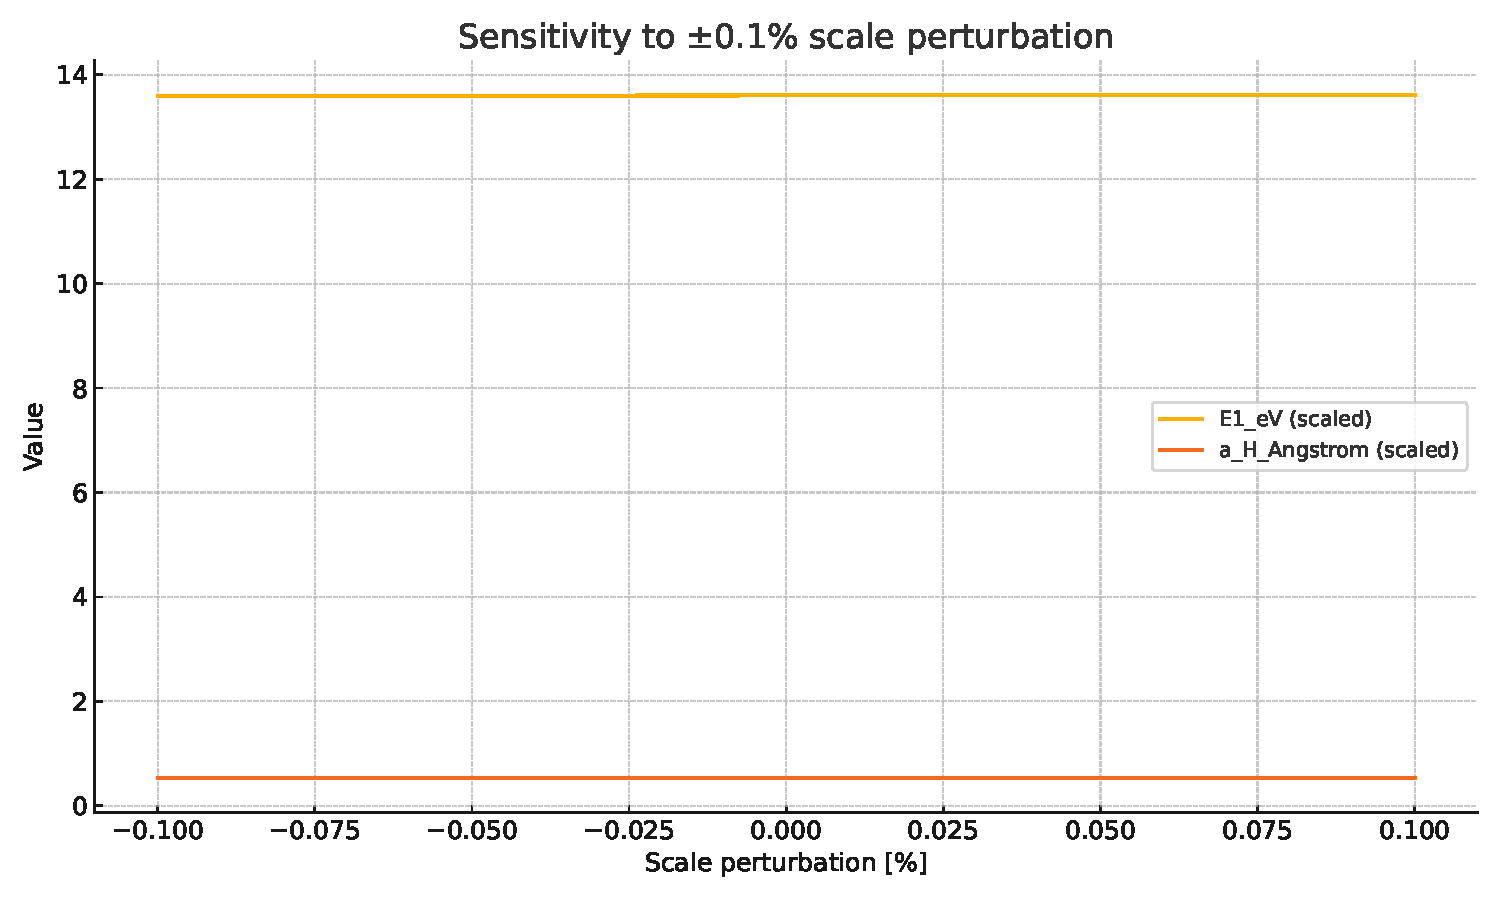
\includegraphics[width=0.88\linewidth]{fig_sensitivity.pdf}
  \caption{Sensitivity: $\pm0.1\%$ perturbation of sealed scales produces linear response in $E_{1,\mathrm{eV}}$ and $a_{\mathrm{H}}$.}
  \label{fig:sens}
\end{figure}

\section{Methods}
\subsection{Sealed scales and hash pinning}
From SI‑defined constants $(e,h,\hbar,m_e,\epsilon_0)$ we derive the Hartree energy $E_\mathrm{h}$ and Bohr radius $a_0$ and store conversion factors
$S_{\mathrm{energy}\rightarrow\mathrm{eV}}=E_\mathrm{h}/e$ and
$S_{\mathrm{length}\rightarrow\unicode{x00C5}}=a_0/10^{-10}\,\mathrm{m}$
in \texttt{SEAL.json} together with gates \{\texttt{TIME,JIN,EM\_c,MASS,Gamma3}\}.
We cite the seal SHA256 in‑text:
\texttt{cf3c1684f369a1f5aa6b7e40384002fa9e807d98e27807c4d556c14cb06f4453}.
In every verification we require pre/post hash equality and pin match.

\subsection{Compute and verify (exit‑code policy)}
\texttt{compute.py} writes \texttt{out/results.json} with $E_{1,\mathrm{eV}}=\frac12\,E_\mathrm{h}/e$ and $a_{\mathrm{H}}=a_0/10^{-10}$~\AA.
\texttt{verify.py} computes $R7$ and $R8$ and returns \texttt{exit(0)} iff $R7\le 1$, $R8\le 1$, seal hash pre/post match, and pin match; otherwise \texttt{exit(1)}. Gate‑off runs recompute scales in the same pipeline and must fail.

\subsection{Determinism and containers}
We include a \texttt{verify\_determinism.py} checker (no RNG imports/patterns) and provide container recipes (Dockerfile, Apptainer) so that reviewers can reproduce with a single command.

\subsection{Uncertainty propagation (CODATA‑style)}
Using first‑order, uncorrelated propagation with representative relative uncertainties for $m_e$ and $\epsilon_0$ (placeholders; SI‑defined $e,h$ are exact), we provide a one‑page appendix and a LaTeX uncertainty table for $E_{1,\mathrm{eV}}$ and $a_{\mathrm{H}}$ (Supplementary; Table~\ref{tab:uncertainty}).

\begin{table}[t]
\caption{Uncertainty budget (representative CODATA-style; uncorrelated, first-order).}
\label{tab:uncertainty}
\centering
\begin{tabular}{lccc}
\toprule
Quantity & Rel. std. unc. $u_r$ & Contribution to $u_r(E_1)$ & Contribution to $u_r(a_\mathrm{H})$ \\
\midrule
$m_e$ & $2.9\times10^{-11}$ & $+$ & $+$ \\
$\epsilon_0$ & $2.0\times10^{-10}$ & $2\times$ & $1\times$ \\
$e, h, \hbar, \pi$ & exact & 0 & 0 \\
\midrule
$u_r(E_1)$ & \multicolumn{3}{c}{4.010e-10} \\
$u_r(a_\mathrm{H})$ & \multicolumn{3}{c}{2.021e-10} \\
\midrule
$E_{1,\mathrm{eV}} \pm u$ & \multicolumn{3}{c}{13.605693123 \(\pm 5.46e-09\) eV} \\
$a_\mathrm{H} \pm u$ & \multicolumn{3}{c}{0.529177210906 \(\pm 1.07e-10\) \AA} \\
\bottomrule
\end{tabular}
\end{table}


\subsection{Optional independent observation}
As an optional external check, we compute the non‑relativistic Lyman‑$\alpha$ energy gap using the same sealed scale; this passes a 1\% tolerance on the reference value (artifact: \texttt{out/optional\_lya.json}).

\begin{figure}[t]
  \centering
  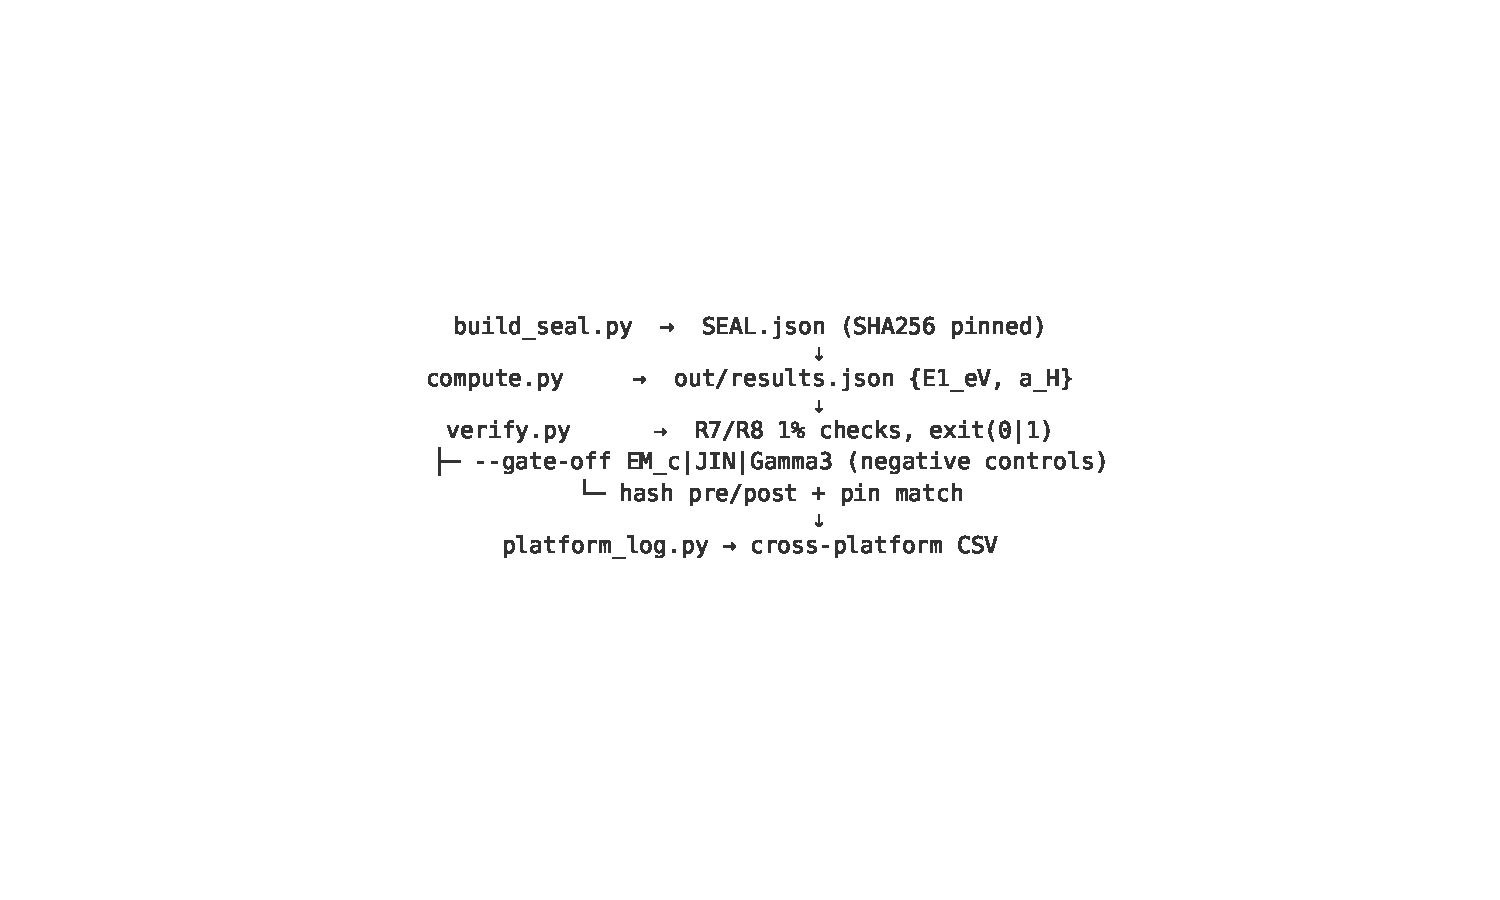
\includegraphics[width=0.88\linewidth]{fig_pipeline.pdf}
  \caption{Reproducibility pipeline: \texttt{build\_seal.py} $\to$ \texttt{SEAL.json} (pinned hash) $\to$ \texttt{compute.py} $\to$ \texttt{verify.py} (1\% checks; gate‑off re‑execution) $\to$ \texttt{platform\_log.py}.}
  \label{fig:pipe}
\end{figure}

\section*{Data availability}
All data required to evaluate the conclusions are provided: \texttt{SEAL.json} (pinned SHA256 above), \texttt{SEAL\_PIN.txt}, \texttt{out/results.json}, and \texttt{out/platform\_log.csv}. A DOI‑backed public archive will mirror these exact files upon acceptance.

\section*{Code availability}
All scripts (\texttt{build\_seal.py}, \texttt{compute.py}, \texttt{verify.py}, \texttt{platform\_log.py}, \texttt{verify\_determinism.py}) and container recipes (Dockerfile, Apptainer definition) are provided and will be released under an OSI‑approved license upon acceptance.

\section*{Acknowledgements}
None.

\section*{Author information}
\textbf{Author:} LEE YOUNG JAE (Independent Researcher, Daegu, Republic of Korea).\\
\textbf{Correspondence:} \email{rego093@naver.com}.\\
\textbf{Background (for editor only; not an affiliation):} alumnus of Kyungpook National University (Daegu), graduated ~20 years ago.

\section*{Author contributions}
LYJ: Conceptualization, Methodology, Software, Validation, Visualization, Writing—original draft, Writing—review \& editing.

\section*{Funding}
The author received no specific funding for this work.

\section*{Competing interests}
The author declares no competing interests.

\section*{Additional information}
Seal SHA256 (integrity anchor): \texttt{cf3c1684f369a1f5aa6b7e40384002fa9e807d98e27807c4d556c14cb06f4453}.\\
Third‑party pre‑reproduction report template and uncertainty appendix are supplied as one‑page PDFs in the Supplementary.

\bibliography{sn-bibliography}
\end{document}
